\section{Radial geometry and regional accounts}\label{sec:account}
\subsection{Diagnostic balls and complete profiles}\label{sec:radial}
Let $\xi=s-s_0\in[-L_c/2,L_c/2]$, with seam endpoints identified. The radial distance from $O$ is
\begin{equation}\label{eq:radial}
 D(\xi)^2=|\gamma(s)-O|^2
 =K_c^2+\RG^2-2K_c\RG\cos(\xi/\RG).
\end{equation}
Since $K_c/\RG=(2+\sqrt3)/\sqrt7>1$, its minimum and maximum are $D_{\min}=K_c-\RG>0$ and $D_{\max}=K_c+\RG$. Moreover,
$\mathrm d(D^2)/\mathrm d|\xi|=2K_c\sin(|\xi|/\RG)>0$ for $0<|\xi|<L_c/2$. Thus $s_0$ is the unique nearest point. Increasing $s$ approaches $O$ on one half and recedes on the other; this geometric orientation does not prescribe the sign of $j$.

\begin{proposition}[Ball preimages and containment]\label{prop:ball}
For the closed ball $\overline B(O,R_B)$, the preimage on the carrier is empty when $0\le R_B<D_{\min}$, is $\{s_0\}$ when $R_B=D_{\min}$, and is the whole circle when $R_B\ge D_{\max}$. For $D_{\min}<R_B<D_{\max}$ it is
\begin{equation}\label{eq:halfarc}
 I_{R_B}=[s_0-A_{R_B},s_0+A_{R_B}],\qquad
 A_{R_B}=\RG\arccos\!\left(\frac{K_c^2+\RG^2-R_B^2}{2K_c\RG}\right),
 \quad 0<A_{R_B}<L_c/2.
\end{equation}
In this intermediate case,
\begin{equation}\label{eq:containment}
 \Sb\subset I_{R_B}\quad\Longleftrightarrow\quad A_{R_B}\ge\eta_g+\epsc.
\end{equation}
\end{proposition}
\begin{proof}
The preimages follow by inverting the strictly increasing distance on either side of $s_0$. The largest absolute offset in \eqref{eq:supports} is $\eta_g+\epsc<2\eta_g<L_c/2$, proving \eqref{eq:containment} including equality.
\end{proof}

The arc length $2A_{R_B}$ may exceed half the circumference. For an open ball the nearest equality is empty, intermediate endpoints are omitted, and at $R_B=D_{\max}$ only the far point is omitted. These null-set changes leave storage integrals unchanged. Tangencies are not two distinct transverse cuts. Equality in \eqref{eq:containment} includes the zero-valued tent endpoints in the closed ball; for an open ball it gives zero forcing outside almost everywhere but not literal containment of the closed supports. At $A_{R_B}=\eta_g$ the contact centers themselves are cuts, and each positive-width profile straddles its cut.

The original close sphere of the folded host has radius
\begin{equation}\label{eq:closesphere}
 R_0=\sqrt{\frac{13}{12}-\frac{\sqrt2}{2}},\qquad
 A_0=A_{R_0},\qquad \epsilon_{\max}=A_0-\eta_g.
\end{equation}
The host construction gives $R_0^2=1/12+1/4+h_g^2$ \cite{PG}. Exact rational radical enclosures in the accepted central-route record establish
\begin{equation}\label{eq:closemargins}
 R_0^2-2a_c^2>\frac4{100},\qquad
 K_c^2+\RG^2+\frac{2K_c\RG}{7}-R_0^2>\frac{59}{100}.
\end{equation}
Since $D(\eta_g)^2=2a_c^2$ and $\cos(2\theta_g)=-1/7$, monotonicity then gives
\begin{equation}\label{eq:widthceiling}
 \eta_g<A_0<2\eta_g,\qquad 0<\epsilon_{\max}<\eta_g,\qquad
 \Sb\subset I_{R_0}\quad\Longleftrightarrow\quad 0<\epsc\le\epsilon_{\max}.
\end{equation}
Thus $\epsc<\eta_g$ alone does not ensure close-sphere containment. No working width or material wall is selected by this comparison.

\begin{table}[htbp]\centering\small
\caption{Illustrative width-one lengths, rounded. Exact formulas control the claims; these are not certified decimal endpoints.}\label{tab:lengths}
\begin{tabular}{lr@{\qquad}lr}\toprule
Quantity & Value & Quantity & Value\\\midrule
$D_{\min}$ & $0.220257905810$ & $\eta_g$ & $0.459778043861$\\
$\sqrt2a_c$ & $0.573491414879$ & $A_0$ & $0.499891808831$\\
$R_0$ & $0.613373093758$ & $\epsilon_{\max}$ & $0.040113764970$\\
$D_{\max}$ & $1.293162100177$ & & \\\bottomrule
\end{tabular}
\end{table}

\begin{figure}[!htbp]\centering
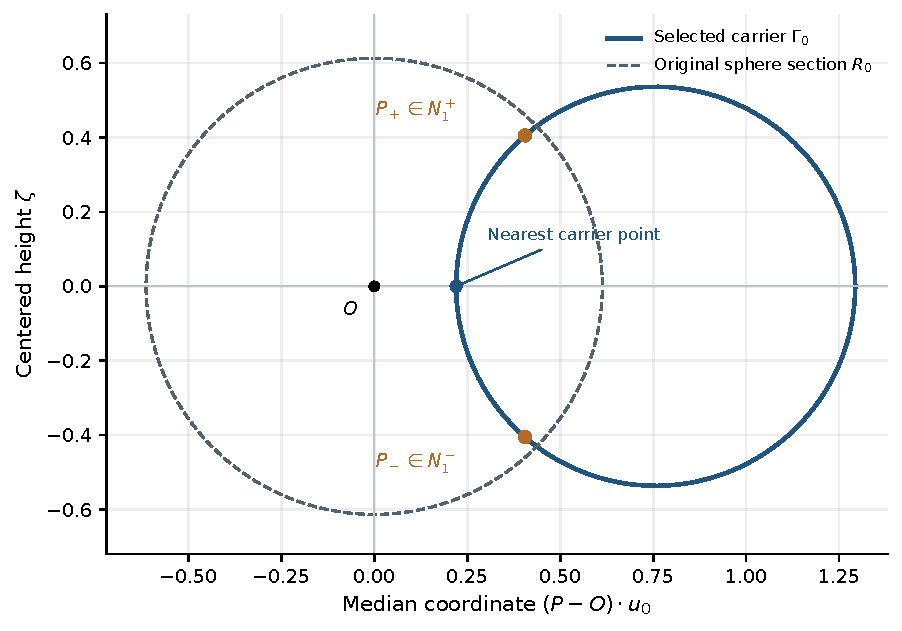
\includegraphics[width=0.78\textwidth]{figures/central_route.pdf}
\caption{The selected carrier in its median plane at width one. The dots are its actual $N_1^\pm$ contact centers; the nearest point remains distinct from $O$. The dashed circle is the original close-sphere section of radius $R_0$, a diagnostic comparison. No profile width, material wall, energetic cone or direction of flow is chosen.}\label{fig:radial}
\end{figure}

\subsection{Cut signs, complementary work and native jumps}\label{sec:regional}
For an intermediate ball let $\ell=s_0-A_{R_B}$, $r=s_0+A_{R_B}$, and define
\begin{equation}\label{eq:regionaldefinitions}
 E_B(t)=\int_\ell^r e(s,t)\dd s,\qquad
 P_L=-j(\ell,t),\quad P_R=j(r,t),\quad P_\partial=j(r,t)-j(\ell,t).
\end{equation}
The signs express outward orientation of the one-dimensional interval: increasing $s$ enters at $\ell$ and leaves at $r$. No obliquity multiplier enters this carrier account. With $H^1$ spatial fields, the cuts have traces and the weak product rule gives
\begin{equation}\label{eq:localregional}
 \dot E_B=-P_\partial+\int_{I_{R_B}}pBq\dd s,\qquad
 \dot H_N+\dot H_R=-\int_0^{L_c}pBq\dd s.
\end{equation}
For arbitrary $L^2$ carrier preparation the global port work still makes sense, but these point-cut statements do not follow from $L^2$ alone.

\begin{proposition}[Exact regional account]\label{prop:regional}
On a finite exchange or hybrid window whose endpoints are evaluated after any jump at that endpoint,
\begin{equation}\label{eq:regionalbalance}
 \begin{aligned}
 &[H_N+H_R+E_B]_{t_a}^{t_b}\\
 &\quad=\mathcal B_N(t_a,t_b)
 -\int_{t_a}^{t_b}P_\partial(t)\dd t
 -\int_{t_a}^{t_b}\int_{I_{R_B}^{c}}p(s,t)Bq(s,t)\dd s\dd t,\\
 &\mathcal B_N(t_a,t_b)=\sum_{t_a<t_n\le t_b}b_n.
 \end{aligned}
\end{equation}
For pure exchange $\mathcal B_N=0$.
\end{proposition}
\begin{proof}
Add \eqref{eq:localregional}. The integral over $I_{R_B}$ cancels only that part of the global port work, leaving the complementary integral with a minus sign. Integrate on every exchange segment, then add the native increments \eqref{eq:hybrid}; the other two stores do not jump. The stated endpoint convention includes the right endpoint's jump and excludes the left endpoint's jump.
\end{proof}

Equivalently, if a sampled window is taken from $0^-$ to $(Nh_{\rm ex})^-$, before the respective jumps, it includes $b_0,\ldots,b_{N-1}$. This is the actual native increment sum, rather than a hypothetical exchange-only baseline \cite{RX,F}.

Complete-profile containment makes the last term of \eqref{eq:regionalbalance} vanish. If containment fails, the complementary work is generally present; its sign can vary and special preparations can make it cancel. Suppressing it universally would change the account. Finally, adding $H_N$ and $H_R$ to $E_B$ is an accounting grouping: neither lumped store has thereby acquired a material location inside the diagnostic ball.
